\section{Background}

Execution detouring is widely used throughout the industry with established library implementations already existing. As well as considering related work and why they do not meet our requirements, this section will discuss common methods of detouring. We will also provide the intuition for many of the design decisions of the project by covering the relevant technical details of an executable's life cycle.

\subsection{Detouring}

From a simplified technical viewpoint, a detour is set by replacing the first few instructions of a target function with an unconditional jump to a user-provided detour function. In this way the code path can be redirected for all given calls to some function.

\begin{parcolumns}[nofirstindent]{2}
 \colchunk{
  \noindent\begin{minipage}{.45\textwidth}

\begin{lstlisting}[language={[x86masm]Assembler},caption={Original code},label={lst:OrigCode},columns=fixed]
TargetFunction:
  PUSH EBP $\tikzmark{L1line1}$
  MOV EBP, ESP
  SUB ESP, 0x0C0
  PUSH EBX $\tikzmark{L1line2}$
  PUSH ESI
  ...
  RET
\end{lstlisting}

  \end{minipage}
 }
 \colchunk{
  \begin{minipage}{.45\textwidth}

\begin{lstlisting}[language={[x86masm]Assembler},caption={Code after insertion of detour},label={lst:AfterDetour},columns=fixed]
TargetFunction:
$\tikzmark{L2line1}$  JMP Instrumentation
  NOP
  NOP
  NOP
  NOP
$\tikzmark{L2line2}$  PUSH EBX
  PUSH ESI
  ...
  RET

Instrumentation:
  ...
  RET
\end{lstlisting}

  \end{minipage}
 }
 \colplacechunks
\end{parcolumns}

\tikz[overlay,remember picture,-latex] \draw[dashed,thick,out=0,in=160,color=black,->] ($(L1line1)+(0pt,0.7ex)$) to ($(L2line1)+(0pt,0.7ex)$);
\tikz[overlay,remember picture,-latex] \draw[dashed,thick,out=0,in=200,color=black,->] ($(L1line2)+(0pt,0.7ex)$) to ($(L2line2)+(0pt,0.7ex)$);

\emph{Listing \ref{lst:OrigCode}} and \emph{\ref{lst:AfterDetour}} illustrate a detouring example in x86-32. The x86-64 implementation is conceptually identical but has minor technicalities that must be considered. Both architectures use variable length instructions, which poses a problem for code patching. On x86-32, the \textbf{JMP} instruction is five bytes long and in this example, patching it in places a new instruction boundary between the \textbf{SUB ESP, 0x0C0} and \textbf{PUSH EBX} instructions. The \textbf{SUB ESP, 0x0C0} instruction is partially overwritten, and its preceding instructions completely overwritten. For clarity, we have padded the bytes after the \textbf{JMP} up to the immediately subsequent instruction with \textbf{NOP} even though this is not functionally necessary. The padding has replaced the end of the partially overwritten instruction which would otherwise contain garbage bytes.

When a function is called, the address of the instruction after the \textbf{CALL} is pushed on the stack as the return address. Since the new code does not modify the stack, \emph{Instrumentation} will return using the original return address from the call to \emph{TargetFunction}.

Other methods of detouring exist but are less widely used. For example, instead of patching the target function, all calls to it can be replaced instead. However, to be reliable this technique requires substantial symbolic information which is not commonly available at the binary level.

\subsubsection{Trampoline} \label{sec:trampoline}
Trampolining provides access to the original function by first executing the overwritten instructions and then unconditionally branching to the remainder of the target function. Hence, a detour either replaces the target function or extends its semantics by invoking the original function as a subroutine through the use of the trampoline.

\begin{parcolumns}[nofirstindent]{2}
 \colchunk{
  \noindent\begin{minipage}{.45\textwidth}

\begin{lstlisting}[language={[x86masm]Assembler},caption={Original code},columns=fixed]
TargetFunction:
  PUSH EBP $\tikzmark{L3line1}$
  MOV EBP, ESP
  SUB ESP, 0x0C0
  PUSH EBX $\tikzmark{L3line2}$
  PUSH ESI
  ...
  RET
\end{lstlisting}

  \end{minipage}
 }
 \colchunk{
  \begin{minipage}{.45\textwidth}

\begin{lstlisting}[language={[x86masm]Assembler},caption={Code after insertion of detour with trampoline},label={lst:AfterTrampoline},columns=fixed]
TargetFunction:
  JMP Instrumentation
  NOP ; TargetFunction + 5
  NOP
  NOP
  NOP
$\tikzmark{L4line2}$  PUSH EBX
  PUSH ESI
  ...
  RET

Instrumentation:
  ...
$\tikzmark{L4line1}$  PUSH EBP
  MOV EBP, ESP
  SUB ESP, 0x0C0
  JMP TargetFunction + 5
\end{lstlisting}

  \end{minipage}
 }
 \colplacechunks
\end{parcolumns}

\tikz[overlay,remember picture,-latex] \draw[dashed,thick,out=0,in=160,color=black,->] ($(L3line1)+(0pt,0.7ex)$) to ($(L4line1)+(0pt,0.7ex)$);
\tikz[overlay,remember picture,-latex] \draw[dashed,thick,out=0,in=200,color=black,->] ($(L3line2)+(0pt,0.7ex)$) to ($(L4line2)+(0pt,0.7ex)$);

To provide trampolining functionality, some form of disassembling must occur. We must be able to calculate how many \emph{whole} instructions have been replaced by the \textbf{JMP} instruction. The reason for this is that it must be ensured that the destination of the trampoline's \textbf{JMP} is not to the middle of an instruction as seen with \emph{Listing \ref{lst:AfterTrampoline}}. As well as providing us with the instruction boundary, it is critical for us to know what instructions have been overwritten by the hook. Different instructions are relocated to the trampoline in a different way, such as relative jumps where it is not a simple case of copying bytes.

\subsection{Executable Life Cycle}

To approach the design of a suitable solution in a logical and methodical manner, it is essential to understand certain stages in the life cycle of an executable under Linux. 

\subsubsection{Compiling}
Compilation marks the inception of a program, with the compiler providing the translation from the source file/s to an executable object file. The following is not intended as a comprehensive definition of compilation, but rather the conceptual fundamentals relevant to us.

\paragraph{Static Linking}
When multiple \emph{.c} source files are compiled, each one is first preprocessed (\emph{cpp}) to generate intermediate \emph{.i} files, then compiled by the C compiler (\emph{cc1}) producing \emph{.s} files, which are assembled (\emph{as}) into \emph{.o} relocatable object files. Since we have defined our scope outside of these stages, it is unnecessarily to look at them in further detail. On the other hand, linking stage is more interesting to us since some detouring methods emulate it to add code to the final executable. Static linking combines various relocatable object files to form the final executable object file. The process consists of two tasks\cite{computer_systems}:

\begin{enumerate}
 \item \textbf{Symbol resolution} - Object files typically contain three types of symbols:
  \begin{enumerate}
   \item \textbf{Defined symbols} - These allow other modules to call functions within the module defining the symbols.
   \item \textbf{Undefined symbols} - These occur where the module calls other modules where the symbols are defined.
   \item \textbf{Local symbols} - Used internally within the object file to allow functions to call each other and for the resulting code to be relocatable.
  \end{enumerate}

  The linker is responsible for collating all the symbols and ensuring a symbol reference is associated with exactly one definition. For linking to occur successfully, relocatable object files contain symbol tables which hold information about what symbols are defined and referenced by each module. It should be noted that the symbol table is often stripped fully or at least partially after the linking process.

 \item \textbf{Relocation} - The compiler and assembler do not know where an object will reside in the final executable so generate code and data sections that start at address 0. The linker needs to \emph{relocate} these sections, associating a memory location with each symbol definition. All symbol references then need to be updated to point to the assigned memory location. Relocation merges sections of the same type. For example the \emph{.data} section of the final executable contains the aggregated \emph{.data} sections from each of the input modules.
\end{enumerate}

A common technique in executable editing is to introduce a new object file containing user defined routines to the final executable. This means that references from the original executable to symbols (usually functions) defined in the object file need to be resolved, as do references going the other way (trampolines). Naturally, a relocation stage must also occur but executable editing tools tend to avoid the complexity of further aggregation of sections by simply adding a new sections.

\paragraph{Dynamic Linking}

Dynamic linking postpones the resolving of undefined symbols until runtime. The executable contains undefined symbols, and a list of objects or libraries that will provide definitions to these. These objects are loaded at runtime and a final linking performed. Dynamic linking is a common technique for runtime detouring because of the ease of development. A shared object can be made with the same ease as a regular executable and the Linux loader will handle all the linking.

\paragraph{Position-Independent Code (PIC)}
\label{par:PIC}

Shared objects need to be compiled such that they can be loaded and executed at any address. Such code is called position-independent code and can be generated with a simple \emph{GCC} option (\emph{-fPIC}). Although function addresses can be looked up at runtime by callers, the ELF system uses lazy binding which defers the binding of function addresses until the first time the function is called. The implication of this for modifying an existing binary to make calls to a new shared library is that our library would need to modify data structures within the executable (namely \emph{Global Offset Table} and \emph{Procedure Linkage Table}).

\subsection{Approaches to Execution Detouring}

Code modification can be performed at any stage of the compilation process: source, object or binary level. Source level modification allows instrumentation code to be added directly into a program's source file before compilation occurs either by modifying the compiler or by using the preprocessor to insert special code\cite{profiling_unix}. Object level modification involves changing object files between the assembly and linking steps\cite{purify_fast_detection}. However, this requires a modified linker or relinking of the entire program and cannot be applied to programs where object files are unavailable. Since we are only considering executables after compilation, we can assume both source and object files are unavailable. This limits our scope to binary level execution detouring which falls under two categories:

\begin{enumerate}
 \item \textbf{Executable Editing/Static Binary Rewriting} - This concerns the act of patching code into an executable before it is loaded by the operating system. The injected code is designed for the interception of functions and redirection of code execution.
 \item \textbf{Runtime/Dynamic Detouring} - In this case, the interception code is applied dynamically at runtime, after the operating system has loaded the program into memory.
\end{enumerate}

\begin{figure}[H]
 \centering
 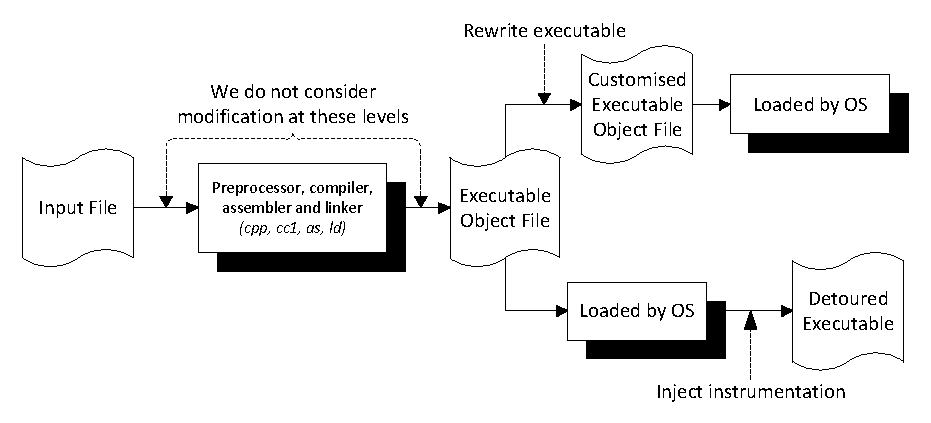
\includegraphics[viewport=21 566 448 757]{Detouring_Options.pdf}
 \caption[Detouring Options]{Our options for inserting instrumentation code. Since we only have access to the executable in its final compiled form, we focus solely on binary level options.}
\end{figure}

\subsubsection{Executable Editing vs Runtime Detouring}

Also known as static code annotation\cite{static_code_annotation}, executable editing is seen as the most convenient to the end user because a single command can be applied to one executable file generating a customised program which can be easily distributed. In comparison, with runtime detouring we are often required to set up a specific runtime environment which might be difficult to use and deploy. In the cases where the production system is on a cloud system such as EC2, this means reconfiguring many environments.

However, the attractiveness of executable editing is reduced when considering the complexity of implementation. Despite being conceptually trivial, executable editing is complex to implement in practice because of architectural and system-specific details. This increases the time and effort required to produce such a tool. Furthermore, at the binary level, symbol-table information is often incomplete and significant analysis must be performed to properly relocate code and data\cite{rewriting_executable_files}.

\subsubsection{Executable Editing}

Conceptually, binary rewriting generally entails a standardised procedure:

\begin{enumerate}
 \item \textbf{Code discovery/analysis} - During this stage, a tool typically analyses the binary and provides an interface to enumerate routines and code blocks which can be split into their constituent instructions. The tool must be able to accurately distinguish between code and data in this case.
\item \textbf{Insertion of instrumentation code} - The insertion stage tends to happen separately and allows insertion/deletion of instructions from the structures discovered in the first stage. It is standard for a tool to allow both the modification of the original binary as well as to provide an option to create a new customised one.
\end{enumerate}

\paragraph{Register Scavenging}

When inserting code to an executable, it is critical not to break the original code by overwriting data or otherwise functionally changing the program in an unintended way. At the assembly language level, this means it is important not to overwrite registers that are in use. Register scavenging uses control flow analysis to provide information about unused registers at any point in a basic block\cite{qpt}. If unused registers can not be found, a last resort is to \emph{push} and \emph{pop} registers to temporarily evict them so they are available for usage.

\paragraph{ELF}

(Executable and Linkable Format) is the file format for executables, object code and shared libraries on Unix-based systems. \emph{libelf} is a library used to directly read, modify and create ELF files in an architecture-independent way. It would be ideal to abstract away from the ELF file format since it is so specific and low-level.

\paragraph{BFD}

(Binary File Descriptor) is a package which allows applications to use the same routines to operate on object files whatever the object file format\cite{bfd}. BFD encapsulates many file formats over many different architectures and presents a common view of them and then provides a unified API to this view. As we will see, some existing Linux binary rewriters build directly over the ELF file format and perform modification through libelf. Although this is a lightweight alternative to BFD, it is undesirable because it locks the code down to a specific file format. Whilst the abstractions BFD provide limit functionality in comparison to dealing with the specific file format directly, it makes it powerful for this precise reason, allowing any library built on top of it to effortlessly and automatically handle differences between and hence support the various formats.

\subsubsection{Runtime Implementation Approaches}

To perform detouring at runtime but achieve the same effect as if it was performed statically, the target must be forced to execute special code as part of its startup - before it starts execution. The purpose of this code is to ensure the instrumentation code is mapped into the target's address space and also to either perform the placement of the detours or implement some system which can perform the detouring dynamically. We now examine different implementation approaches employed by existing tools and research projects.

\paragraph{Shared Library and Position-Independent Code}

Once we have the ability to execute arbitrary code in a target, the placing of the detours at runtime is a trivial matter. The issue we face is how to insert the instrumentation code in the first place and also how to override execution to make sure our special code is run before anything else. One method is to patch the entry point of the target to dynamically load a shared library containing the instrumentation code through the \texttt{dl} interface with functions such as \texttt{dlopen}.  Whilst this does require static insertion of the bootstrapping code, the amount of work required is minimal. One further advantage is that the shared library will already have been compiled to have position-independent code, which means that the Linux loader deals with all the linking of our extra library, something we are required to perform manually with binary rewriting.

GCC conveniently provides a constructor attribute, \texttt{\mbox{void \_\_attribute\_\_ ((constructor))}} which can be used to specify a function which is invoked upon loading of the shared library. With this approach, the constructor would set up the hooks before the main program starts executing:

\begin{lstlisting}[language=C,caption={This example would be compiled as a shared library}]
void init(void) __attribute__ ((constructor));

void init(void)
{
   /*
    * This function is invoked as soon as the library 
    * is loaded. In a dynamic implementation, we would
    * place the code to perform the detours here.
    */
}
\end{lstlisting}

An alternative to patching the executable's entry point to load the bootstrapping library is to use the \texttt{LD\_PRELOAD} environment variable which adjusts the runtime linking process by preloading a shared library into an arbitrary process. Unfortunately, \texttt{LD\_PRELOAD} can be subverted by the application which means this option is unreliable.

\paragraph{Exception Handlers}

Methods used for general debugging often require the breaking or redirection of code flow. One common form of this is breakpointing which comes in two flavours - hardware and software breakpoints. The breakpoint suspends execution before some given instruction is executed and the programmer inspects the program context at that point. As well as inspecting the context, it is possible to modify it, or more specifically the instruction pointer. In the context of a detouring implementation, software breakpoints are often used by replacing instructions with the \texttt{int 3} opcode which when executed triggers an interrupt handler. The interrupt handler can be overridden to modify the EIP/RIP register\cite{fast_breakpoints, profiling_unix, kprobes}.

Similarly, the access protection of memory pages can be changed to become non-executable pages so each access invokes a global exception handler. As with breakpoint trapping, the ability to trap each instruction implies the capability to redirect code flow. Although this approach is interesting, the overhead is too large to be useful in practice.